\renewcommand{\theequation}{\theenumi}
\begin{enumerate}
\numberwithin{equation}{enumi}

\item \begin{align}
\vec{A} &=\myvec{0\\0} \label{eq:constr_a_pts_and_vectors}\\
\vec{B} &=\myvec{36\\15} \label{eq:constr_b_pts_and_vectors}
\end{align}

\item Distance between $\vec{A}$ and $\vec{B}$ is:
\begin{align}
\norm{\vec{A} - \vec{B}} 
\end{align}

\item From the given information:
\begin{align}
\norm{\myvec{0\\0} - \myvec{36\\15}} = 39
\end{align}

\item \begin{figure}[!ht]
\centering
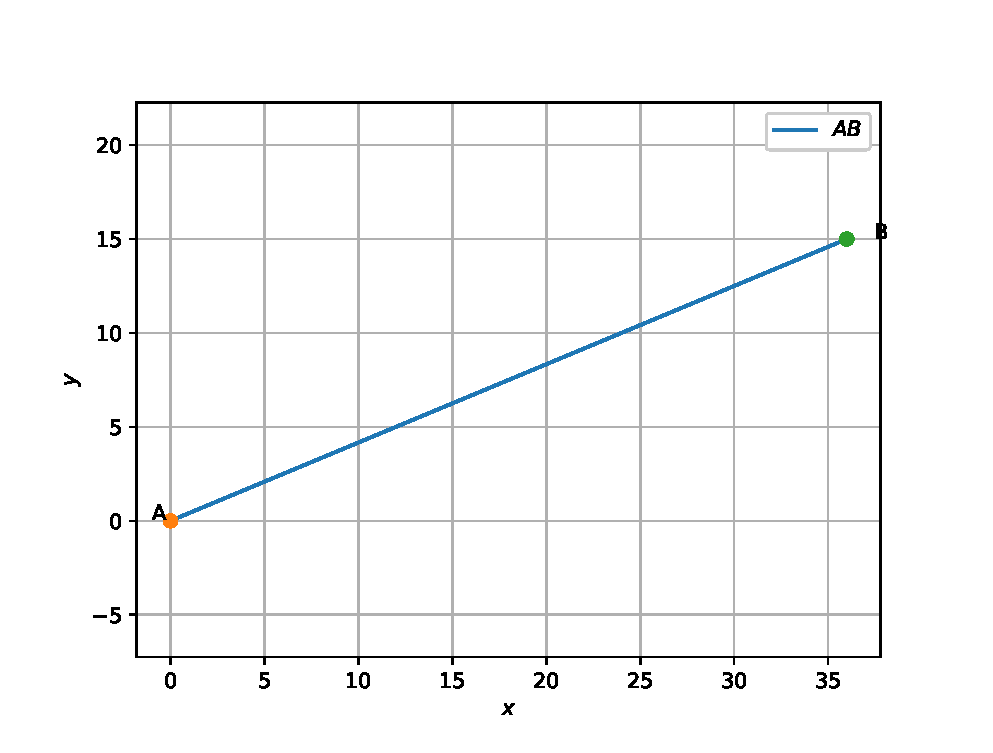
\includegraphics[width=\columnwidth]{./figs/line_ex/pts_and_vectors/dist_bt_pts.eps}
\caption{Line $AB$ generated using python}
\label{fig:dist_btw_pts2_pts_and_vectors}
\end{figure} 

The following Python code generates Fig. \ref{fig:dist_btw_pts2_pts_and_vectors}

\begin{lstlisting}
codes/line_ex/pts_and_vectors/dist_btw_pts.py
\end{lstlisting}

\end{enumerate}





